\chapter{Introduction}
\section{Artificial Neural Networks}

Artifical Neural Networks (ANNs) are a very popular machine learning model. They are known to be very expressive, leading to low statistical bias. With enough neurons, ANNs can approximate any function.  They are especially useful for learning from very large data sets. But it is not entirely clear what the optimization of an ANN converges to, as the loss surface is highly non-convex. Nonetheless a number of results show that for wide enough networks, there are few "bad" local minima.

ANNs are composed of 'neurons', which are in some ways analogous to biological neurons.Each neuron is a nonlinear function transforming the weighted sum of its inputs:
\begin{equation*}
      y = \sigma(w_1x_1+w_2x_2+...+w_nx_n)
\end{equation*}

With $w_i$ the weights, $x_i$ the inputs and $\sigma$ the activation function. This is the McCulloch-Pitts neuron model.[REF] The most commonly used activation function $\sigma$ is the Rectified Linear Unit (ReLU):

\begin{equation*}
      \sigma(x) = x^+ = \max(0,x)
\end{equation*}

A visual representation is shown in figure \ref{neural}b. A full network is built by connecting layers of neurons as shown in figure \ref{neural}a. An ANN can also be expressed as a combination of function composition and matrix multiplication.

\begin{equation*}
         f(W,x) = W_L\sigma(W_{L-1}\sigma(...W_1\sigma(W_0x)...))
\end{equation*}

where $W_n$ are the matrixes of the connection weights and $L$ is the depth of the network. 





   \begin{figure}[b]
	\centering
	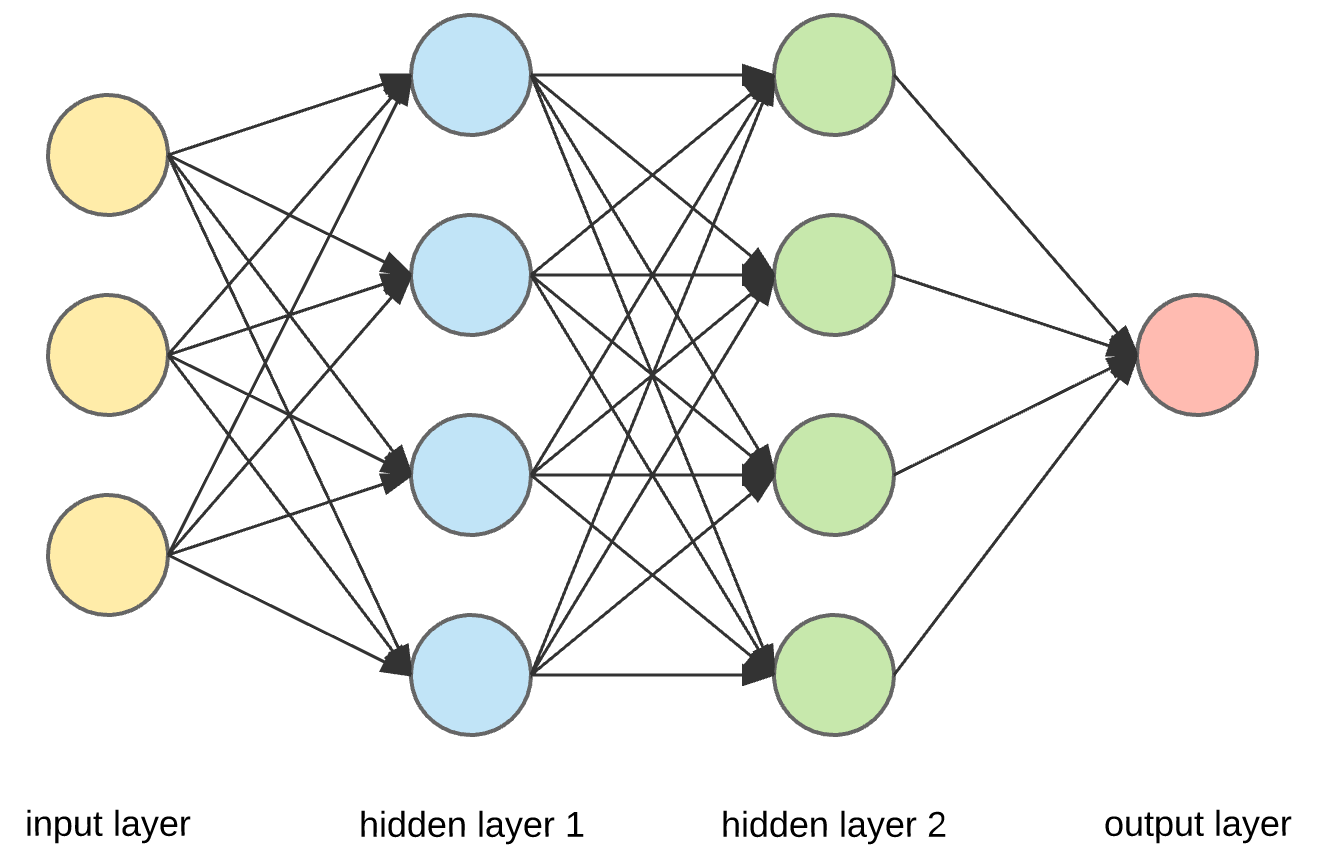
\includegraphics[width=0.49\textwidth]{network}
	%\caption{Feedforward Deep Neural Network. (Retrieved from https://towardsdatascience.com)}
	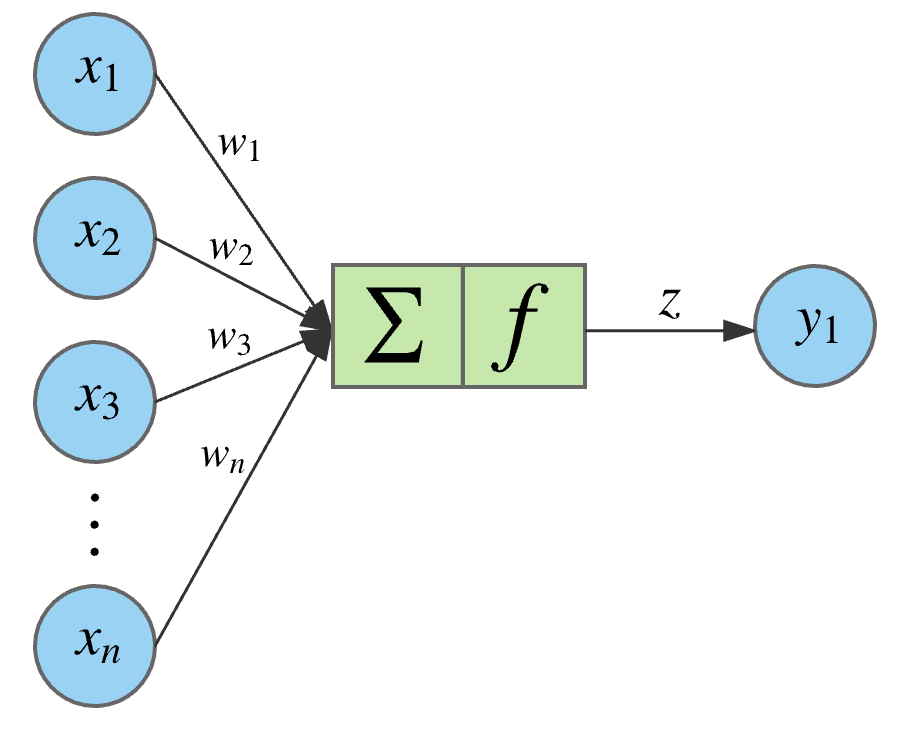
\includegraphics[width=0.49\textwidth]{neuron}
	\caption{Feedforward Deep Neural Network and Single Neuron - McCulloch-Pitts model. (Retrieved from https://towardsdatascience.com)}
	\label{neural}
	\end{figure}

\newpage
\section{Backpropagation}
Backpropagation is the usual algorithm for training an ANN. Training of a network is done by minimizing the loss function $C$. For regression problems this will be often be a squared error loss, while for classification tasks the cross entropy is used.

\begin{equation*}
\begin{aligned}
& \underset{W}{\text{minimize}}
& C(W) &= \sum\limits_{j=0}^{N}||f(W,x^j) - y^j||^2 \\
\end{aligned}
\end{equation*}

with $x^j$ the input vectors, $y^j$ the target output and $N$ the number of data points

Backpropagation computes the gradient of the loss function $C$ with respect to the weight matrices $W$. It has two steps: in the first step the output of the network is calculated using the current weights and input v. The activation values and derivatives of each 
Then the error is propagated backward and the gradient is calculated.

 Then any gradient descent method can be used to find the step update.


\section{Neural Networks in Optimal Control Theory}

\begin{table}
\begin{tabular}{c | c | c }
Optimal Control & Neural Network & Notation\\ \hline
decision variables & weight parameters & $W$\\
state variables & (neuron) activation & $z$\\
\end{tabular}
\end{table}

A neural network can also be interpreted as a dynamical system.
\begin{equation*}
	\begin{aligned}
	z_0 &= x \\
	z_{k+1} &= \sigma(W_kz_k), & k = 0,...,L-1 \\
	y &= W_Hz_L \\
	\end{aligned}
\end{equation*}

In this way optimization methods from control theory can be applied. In particular, training a neural network can be formulated as the following Optimal Control Problem (OCP)

\begin{equation}
	\begin{aligned}
	& \underset{W}{\text{minimize}}
	& & \sum\limits_{j=0}^{N}||W_Lz_L^j - y^j||^2 \\
	& \text{subject to}
	& & z_{k+1}^j = \max(W_kz_k^j,0), &k = 0,\ldots,L-1,j = 1,\ldots,N
	\end{aligned}
	\label{ocp-eq}
\end{equation}


There are two main direct approaches to solving an OCP. First is the sequential approach, where the states are eliminated using the dynamics. This is equivalent to the backpropagation algorithm which is the current standard method. [ref mizutani]

The other approach is the simultaneous approach, where the state variables and the dynamics are kept as constraints. In control theory this approach often works better for highly nonlinear problems, which is certainly the case for training neural networks. The simultaneous approach is novel to neural networks and will be the topic of this thesis.

The disadvantage of this method is the number of variables that need to be optimized is much larger. For a fully connected neural network of width $W$, each layer will contain $W^2$ weights. Combined with a depth $D$, that gives approximately $W^2D$ weight variables to be optimized for both the backpropagation and simultaneous approach. Adding the states as variables however adds another $WDN$ variables, where $N$ is the number of samples in a training batch. The advantage of this method is that relaxing the states makes the problem more smooth, and will hopefully allow the optimization to converge more often to a good solution and not land in a bad local minimum.

\section{Goal of the Thesis}



